\documentclass{beamer}
\usepackage[utf8]{inputenc}
\usepackage[spanish, activeacute]{babel}
\usepackage{caption, subcaption}
\usepackage {amsmath, amssymb, bbm, stackrel, color, colortbl}
\usepackage{tikz}
\definecolor{LightCyan}{rgb}{0.88,1,20}
\definecolor{Gray}{gray}{0.9}
\newcommand{\BigO}[1]{\ensuremath{\operatorname{O}\bigl(#1\bigr)}}

\usetheme{Boadilla}
%\useoutertheme{shadow}

% Para eliminar el footer
%\setbeamertemplate{footline}[page number]{}
% Los navigation symbols no sirven para nada
\setbeamertemplate{navigation symbols}{}

% Para poner la tabla de contenidos automaticamente al comienzo de cada seccion
%\AtBeginSection[]{\begin{frame}\frametitle{Tabla de contenidos}\tableofcontents[currentsection]\end{frame}}

% Customizacion de la tabla de contenidos
%\setbeamerfont{section number projected}{family=\rmfamily,series=\bfseries,size=\normalsize}
%\setbeamercolor{section number projected}{bg=black,fg=yellow}
%\setbeamertemplate{sections/subsections in toc}[ball]


% Title page
\title[Query Expansion with Random Embeddings]{Query Expansion with Random Embeddings}
\author[Lucas Bernardi]{\\[4mm]Lucas Bernardi}
\institute{}
\date{January 2014}


\begin{document}

\frame{\titlepage}

\frame{\tableofcontents}

\section{Intro}

\begin{frame}
	\frametitle{Query Expansion: Problem statement}
	\bigskip
	\begin{itemize}
	\item In the context of Information Retrieval, Query Expansion is a method to improve recall and precision by modifying a user query
  \item A specific case is the expansion of each term to \textit{related} terms, which mainly improves recall but also precision as a side effect
  \item Example: User query: \texttt{soccer}, expanded query: \texttt{soccer football maradona}
  \item  The Problem: \textbf{Learn to expand terms}
	\end{itemize}
\end{frame}

\begin{frame}
	\frametitle{A General Approach}
	\begin{block}{The distributional hypothesis}
    Words with similar distributional properties have similar meanings.
  \end{block}
\bigskip
	\begin{block}{The geometric metaphor of meaning}
  Meanings are locations in a semantic space, and semantic similarity is proximity between the locations.
  \end{block}
\end{frame}


\begin{frame}
	\frametitle{The Vector Space Model Approach}
	\framesubtitle{A solution}
  \begin{itemize}
    \item	An algebraic model for information retrieval and NLP
    \item	Defines a vector space to represent terms
    \item	Defines a dimension for each unique term
    \item	Each term is represented by a semantic vector
    \item Each component of a semantic vector is the weight of the represented term in the direction of the dimension term
    \item Weights are a design decision, TF-IDF is widely used
    \item Compute the related terms of a given term as its k-nearest neighbors
    \item The vector distance/similarity measure is a design decision, cosine similarity is widely adopted
  \end{itemize}
\end{frame}

\begin{frame}
\begin{center}
\small 
\begin{tabular}{|l|l|l|l|l|l|l|l|l|l|}
\hline
~        & play & soccer & week & favorite & sport & forget & ball & Football \\ \hline
play     & 0    & 1      & 1    & 0        & 0     & 0      & 0    & 1        \\ \hline
\rowcolor{LightCyan}
soccer   & 1    & 0      & 1    & 1        & 1     & 1      & 1    & 0        \\ \hline
week     & 1    & 1      & 0    & 0        & 0     & 0      & 0    & 0        \\ \hline
favorite & 0    & 1      & 0    & 0        & 1     & 0      & 0    & 0        \\ \hline
sport    & 1    & 1      & 0    & 1        & 0     & 0      & 0    & 1        \\ \hline
forget   & 0    & 1      & 0    & 0        & 0     & 0      & 1    & 0        \\ \hline
ball     & 0    & 1      & 0    & 0        & 0     & 1      & 0    & 0        \\ \hline
\rowcolor{LightCyan}
Football & 1    & 0      & 0    & 0        & 1     & 0      & 0    & 0        \\ \hline
\end{tabular}

\end{center}
$s(soccer) = \begin{pmatrix} 1 & 0 & 1 & 1 & 1 & 1 & 1 & 0\end{pmatrix} $\\
\medskip
$s(Football) = \begin{pmatrix} 1 & 0 & 0 & 0 & 1 & 0 & 0 & 0 \end{pmatrix} $\\
\medskip
$similarity(soccer, Football)=cos(s(soccer), s(football)) = \frac{1}{\sqrt 3} = 0.57$
\end{frame}

\begin{frame}
	\frametitle{The Vector Space Model Approach}
	\framesubtitle{Some drawbacks}
  \begin{itemize}
    \item	Curse of dimensionality
    \item	Sparse vectors
    \item	Dynamic vector space
      \end{itemize}
      \bigskip
      Alternatives
  \begin{itemize}
    \item	Use documents as dimensions: Less dimensions, but still sparse vectors and still a dynamic space
    \item	Use topics as dimensions: Less dimensions, dense vectors and fixed space, but how can we define topics and assign weights?  Latent Semantic Analysis
  \end{itemize}
\end{frame}

\section{Random Projections}

\begin{frame}
	\frametitle{The Random Projections Approach}
	\framesubtitle{Overcoming drawbacks}
	\begin{itemize}
	\item Use a random low dimensional space
	\item Less dimensions, dense vectors, fixed space
	\item No semantic assigned to dimensions
	\item But, how are weights assigned?
	\end{itemize}
\end{frame}

\begin{frame}
	\frametitle{The Random Projections Approach}
	\framesubtitle{A simple algorithm }
	\begin{itemize}
		\item Assign a random k-dimensional vector to each term (index vector)
		\item Allocate a null k-dimensional vector to each term (semantic vector)
		\item For each sentence in the corpus compute bigrams $(left$ $right)$
		\item For each bigram 
		\begin{itemize}
		  \item $semantic(left)$ += $index(right)$
		  \item $semantic(right)$ += $index(left)$
		\end{itemize}
	\end{itemize}
\end{frame}	


\begin{frame}
	\frametitle{The Random Projections Approach}
	\framesubtitle{Illustration}
\begin{columns}[t]
\begin{column}{0.5\textwidth}
Document 1:\\
We play soccer every week. Soccer is my favorite sport. Don't forget the soccer ball\\
\medskip
Context 1: play soccer week.\\
Context 2: Soccer favorite sport.\\
Context 3: forget soccer ball.\\
\end{column}
\begin{column}{0.5\textwidth}
Document 2:\\
Football is a popular sport. Do you play football?\\
\medskip
Context 1: Football popular sport\\
Context 2: play football
\end{column}
\end{columns}
\bigskip
$s(\texttt{soccer}) = r(\texttt{play}) + r(\texttt{week}) + r(\texttt{favorite}) + r(\texttt{sport}) + r(\texttt{forget}) + r(\texttt{ball}) = $
$\langle 10001 \rangle + \langle 10100 \rangle + \langle 00011 \rangle+ \langle00110 \rangle+ \langle 11000 \rangle+ \langle 10010 \rangle = \langle 41232\rangle $

\medskip
$s(\texttt{football}) =$
$ r(\texttt{popular}) + r(\texttt{sport}) + r(\texttt{play}) = \langle 10010 \rangle + \langle 00110 \rangle + \langle 10001 \rangle = \langle 20121 \rangle$

\medskip
$cos(s(\texttt{soccer}), s(\texttt{football})) = cos(\langle 41232 \rangle, \langle 20121 \rangle) = 0.97$

\end{frame}

\begin{frame}
	\frametitle{The Random Projections Approach}
	\framesubtitle{A simple algorithm: a formal description}

Given a text documents corpus $D$ we define \\
$\mathbb{T}=\{\text{All terms in } D\}$, $t =  \left\vert{\mathbb{T}}\right\vert$ \\
$\mathbb{C} = \{\text{All contexts in } D\}$, where a context is a set of terms \\
$t$ random $k$-dimensional vectors $r_i, 1\leq i\leq t$,  $\mathbb{R} = \{r_i\}$ \\
$t$ semantic $k$-dimensional vectors $s_i, 1\leq i\leq t$,  $\mathbb{S} = \{s_i\}$ \\
A mapping $S:w \in \mathbb{T} \rightarrow  \mathbb{S}$, which maps a term to its semantic vector \\
A mapping $R:w \in \mathbb{T} \rightarrow  \mathbb{R}$, which maps a term to its random vector \\
A mapping $C:w \in \mathbb{T} \rightarrow  \{\mathbb{C}\}$, which maps a term to a set containing all the contexts it appears \\
Then we can express the semantic vector assigned to the term $w$ as: \\
\begin{equation}
s_w =\sum\limits_{c \in C(w)} \sum\limits_{p \in c} R(p)
\end{equation}
\end{frame}


\begin{frame}
  	\frametitle{The Random Projections Approach}
  	\framesubtitle{Algebraic Interpretation}
  	
Defining a co-occurrence matrix $M \in \mathbb{Z}^{t \times t} $, $M_{ij} = \sum\limits_{c \in C(t_i)} \mathbbm{1}_c (t_j)$ \\
Each cell $i, j$ in $M$ counts the amount of contexts in $D$ containing the $i$th and $j$th terms\\
Introducing a random matrix $R \in \mathbb{Z}^{t \times k} $,  $R_i = R(t_i)$, that is, all random vectors as rows, we can express a semantic vector as:\\
\begin{equation}
s_i =\sum\limits_{j=1}^{t} R(t_j)M_{ij} =\sum\limits_{j=1}^{t} R_jM_{ij}
\end{equation}
If we also define the semantic matrix $S \in \mathbb{Z}^{t \times k} $ with $S_i = s_i$, that is, all semantic vectors as rows, we can finally write:\\
\begin{equation}
S=MR
\end{equation}
\end{frame}


\begin{frame}
  	\frametitle{The Random Projections Approach}
  	\framesubtitle{Algebraic Interpretation}
  	\begin{equation}
S=MR
\end{equation}
\begin{itemize}
  \item This equation is a mathematical expression of our initial algorithm
  \item Semantic vectors are just the matrix product of the VSM vectors and a random matrix
  \item The algorithm is simply reducing the dimensionality of the VSM vectors
  \item For certain distributions of R, R is a nearly orthogonal
  \item Then we can interpret this product as the projection of the VSM vectors onto a random lower dimensional space
\end{itemize}
\end{frame}


\begin{frame}
  	\frametitle{The Random Projections Approach}
  	\framesubtitle{Theoretical support}
  	\begin{block}{The Johnson and Lindenstrauss Lemma}
Given $\epsilon > 0$ and an integer $n$, let $k$ be a positive integer such that $k \geq k_{0} = \BigO{\epsilon^{-2}  \log n} $. For every set $\mathbb{P}$ of $n$ points in $\mathbb{R}^{d}$ there exists $f: \mathbb{R}^{d}  \rightarrow \mathbb{R}^{k}$ such that for all $u,v \in \mathbb{P}$\\
  	\bigskip
  	\centering
  	$(1-\epsilon)\lVert u-v \rVert^{2} \le \lVert f(u)-f(v) \rVert^{2}\le (1+\epsilon)\lVert u-v \rVert^{2}$\\
  	\end{block}
\end{frame}
\begin{frame}
  	\frametitle{The Random Projections Approach}
  	\framesubtitle{Theoretical support}
\begin{block}{Achlioptas Theorem}

  	  Let $\mathbb{P}$ be an arbitrary set of $n$ points in $R^{d}$ represented as an $n \times d$ matrix $A$. Given $\epsilon, \beta >0$ let $k_{0}=\frac{4+2\beta}{\frac{\epsilon^{2}}{2}-\frac{\epsilon^{3}}{3}}\log n$. For integer $k \ge_{0}$, let $\mathbb{R}$ be a $d \times k$ random matrix with $R(i,j)=r_{ij}$, where $\{r_{ij}\}$ are independent random variables from either one of the following two probability distributions:\\

\begin{minipage}[b]{0.45\linewidth}
\[
 r_{i,j} =
  \begin{cases}
   +1 & \text{with probability } \frac{1}{2} \\
  -1 & \text{with probability } \frac{1}{2} \\
  \end{cases}
\]  	  
\end{minipage}
\begin{minipage}[b]{0.45\linewidth}
\[
 r_{i,j} = \sqrt{3}\times 
  \begin{cases}
   +1 & \text{with probability } \frac{1}{6} \\
   0 & \text{with probability } \frac{2}{3} \\
  -1 & \text{with probability } \frac{1}{6} \\
  \end{cases}
\]
\end{minipage}\\
\bigskip
Let $E=\frac{1}{\sqrt{k}}AR$. Let $f: \mathbb{R}^{d}\rightarrow \mathbb{R}^{k}$ map the $i^{th}$ row of $A$ to the $i^{th}$ row of $E$.
\bigskip
With probability at least $1-n^{-\beta}, for all u, v \in \mathbb{P} $

\centering
$(1-\epsilon)\lVert u-v \rVert^{2} \le \lVert f(u)-f(v) \rVert^{2}\le (1+\epsilon)\lVert u-v \rVert^{2}$\\
\end{block}
\end{frame}

\section{Empirical Study}

\begin{frame}
\frametitle{Empirical Study}
\framesubtitle{Set up}
\begin{itemize}
  \item Natural language corpus with 140000 unique terms
  \item Filtered out low frequency terms, $n=42905$
  \item Plain VSM vectors (original space is represented by the co-occurrence matrix)
  \item Evaluated random space dimension ($k_{0}$) ranging from 100 to 2000
  \item Random space generated with the dense Achlioptas distribution
  \item Pick two random vectors $u, v$, compute squared euclidean distance $\lVert u-v \rVert^{2}$ and $\lVert f(u)-f(v) \rVert^{2}$
  \item Compute relative error as $\frac{\lVert f(u)-f(v) \rVert^{2}-\lVert u-v \rVert^{2}}{\lVert u-v \rVert^{2}}$ 
  \item Sample size: $3000$
  \end{itemize}
\end{frame}


\begin{frame}
\frametitle{Empirical Study}
\framesubtitle{Results}
  		\begin{figure}
		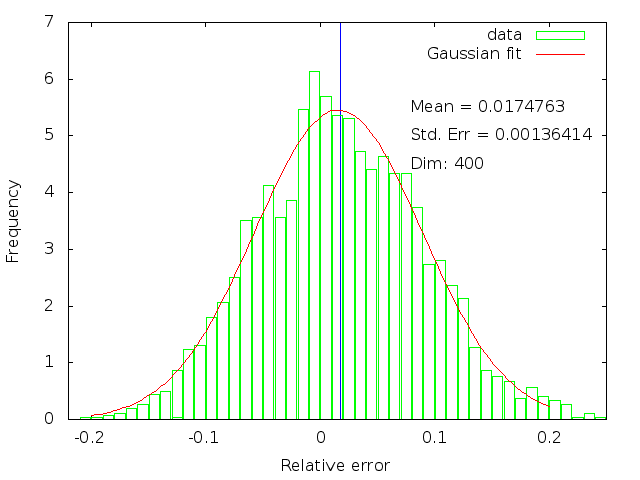
\includegraphics[scale=0.46]{histogram400.png}
	\end{figure}
\end{frame}

\begin{frame}
\frametitle{Empirical Study}
\framesubtitle{Results}
  		\begin{figure}
		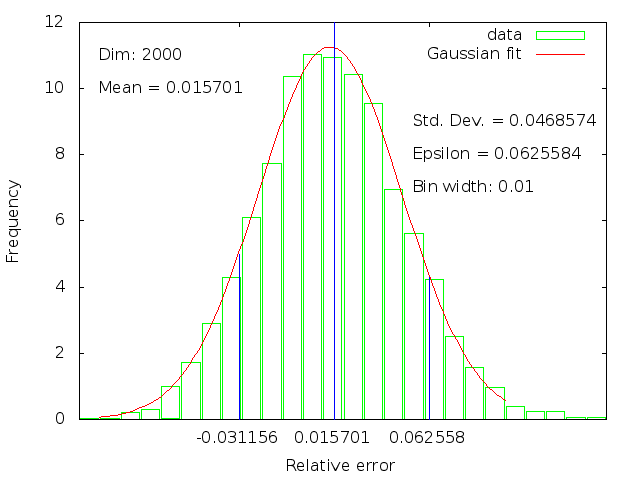
\includegraphics[scale=0.46]{histogram2000.png}
	\end{figure}
\end{frame}

\begin{frame}
\frametitle{Empirical Study}
\framesubtitle{Results}
  		\begin{figure}
		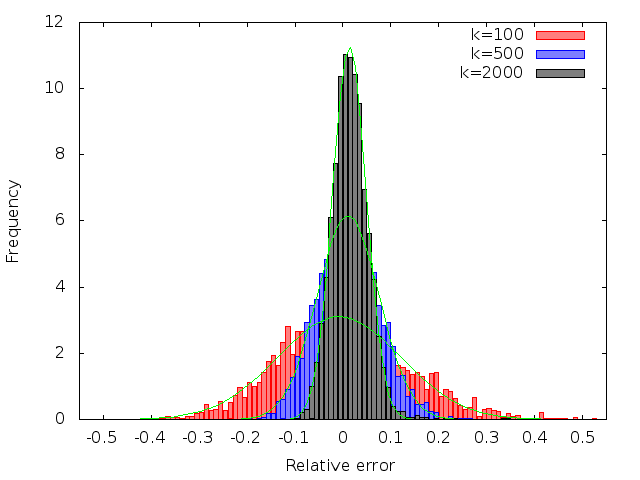
\includegraphics[scale=0.46]{histogramAll.png}
	\end{figure}
\end{frame} 

\begin{frame}
\frametitle{Empirical Study}
\framesubtitle{Measuring $\epsilon$}

How can we compute $\epsilon$ from these histograms?
\medskip
\begin{center}
$(1-\epsilon)\lVert u-v \rVert^{2} \le \lVert f(u)-f(v) \rVert^{2}\le (1+\epsilon)\lVert u-v \rVert^{2}$\\
\medskip
$1-\epsilon \le \frac{\lVert f(u)-f(v) \rVert^{2}}{\lVert u-v \rVert^{2} }\le 1+\epsilon$\\
\medskip
$-\epsilon \le \frac{\lVert f(u)-f(v) \rVert^{2}}{\lVert u-v \rVert^{2}} - 1\le \epsilon$\\
\medskip
$-\epsilon \le \frac{\lVert f(u)-f(v) \rVert^{2}-\lVert u-v \rVert^{2}}{\lVert u-v \rVert^{2}}\le \epsilon$\\
\medskip
$\epsilon = \max(\lvert \mu - \sigma\rvert, \lvert \mu + \sigma\rvert)$\\
\end{center}


\end{frame}

\begin{frame}
\frametitle{Empirical Study}
\framesubtitle{Results}

\footnotesize
\begin{tikzpicture}
    \draw (0, 0) node[inner sep=0] {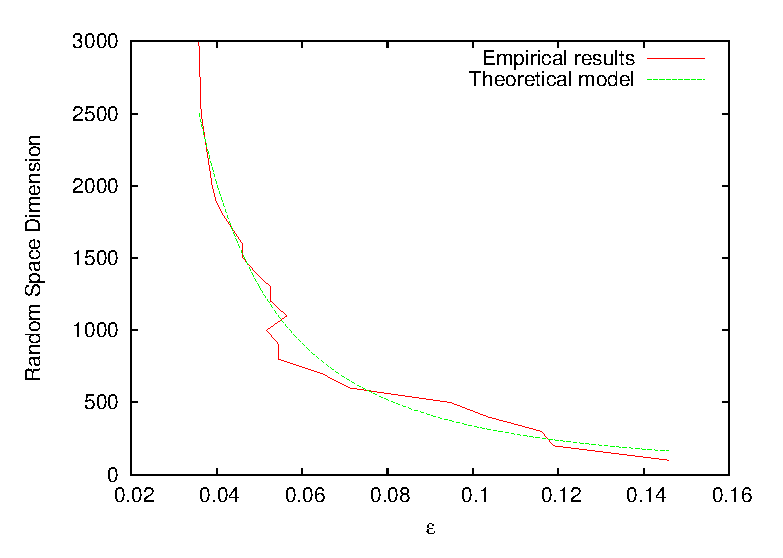
\includegraphics[scale=0.85]{epsilon.eps}};
    \draw (0, 2) node{$k_{0}=\frac{4+2\beta}{\frac{\epsilon^{2}}{2}-\frac{\epsilon^{3}}{3}}\log n $};
\end{tikzpicture}

\end{frame} 
\begin{frame}
\frametitle{Empirical Study}
\framesubtitle{Computing $\beta$}
\footnotesize
\begin{tikzpicture}
    \draw (0, 0) node[inner sep=0] {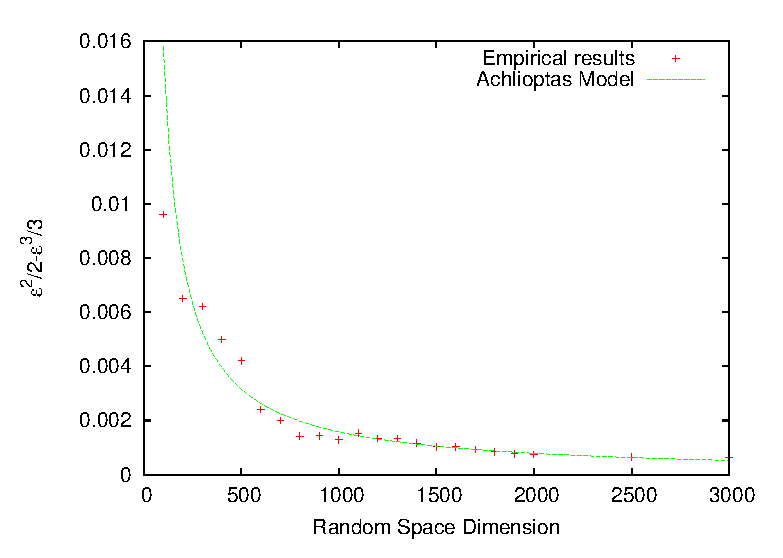
\includegraphics[scale=0.9]{epsilonFit.eps}};
    \draw (0, 2) node{Achlioptas Model: $k_{0}=\frac{4+2\beta}{\frac{\epsilon^{2}}{2}-\frac{\epsilon^{3}}{3}}\log n \Rightarrow$};
    \draw (1, 1) node {$\frac{\epsilon^{2}}{2}-\frac{\epsilon^{3}}{3}=\frac{4+2\beta}{k_{0}}\log n$};
\end{tikzpicture}
\end{frame} 

\begin{frame}
\frametitle{Empirical Study}
\framesubtitle{Computing $\beta$}
\footnotesize
\begin{tikzpicture}
    \draw (0, 0) node[inner sep=0] {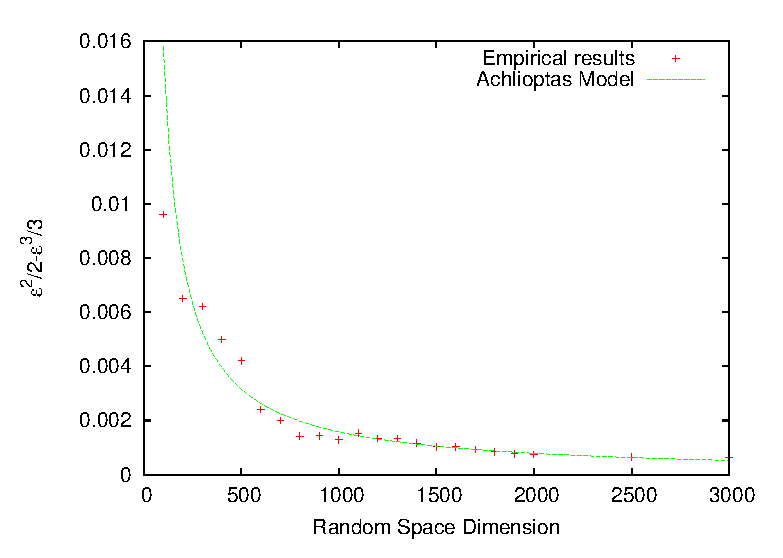
\includegraphics[scale=0.9]{epsilonFit.eps}};
    \draw (0, 2) node{Achlioptas Model: $k_{0}=\frac{4+2\beta}{\frac{\epsilon^{2}}{2}-\frac{\epsilon^{3}}{3}}\log n \Rightarrow$};
    \draw (1, 1) node {$\frac{\epsilon^{2}}{2}-\frac{\epsilon^{3}}{3}=\frac{4+2\beta}{k_{0}}\log n$};
    \draw (1, 0) node {$\beta=0.269, Pr(\epsilon) = 1-n^{-\beta} = 1-42905^{-0.269}=0.94$};
\end{tikzpicture}
\end{frame} 

\begin{frame}
\frametitle{Empirical Study}
\framesubtitle{Sparse projections}

\footnotesize
\begin{tikzpicture}
    \draw (0, 0) node[inner sep=0] {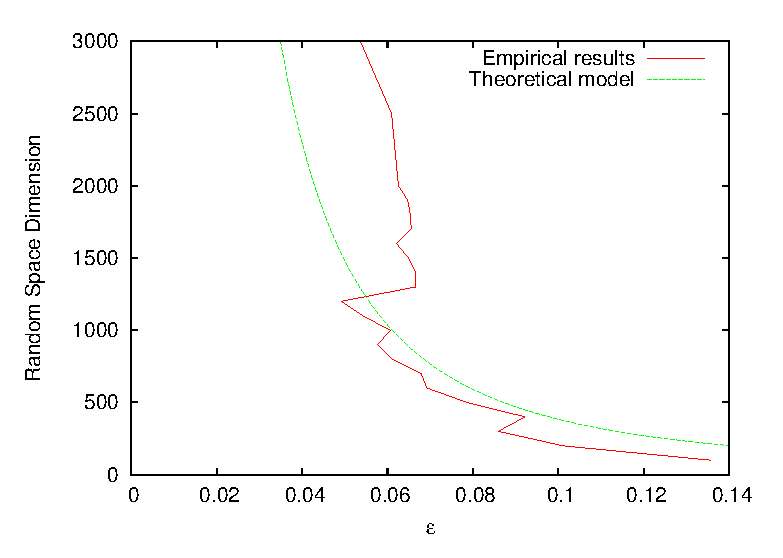
\includegraphics[scale=0.85]{epsilon-sparse.eps}};
    \draw (2, 2) node{$k_{0}=\frac{4+2\beta}{\frac{\epsilon^{2}}{2}-\frac{\epsilon^{3}}{3}}\log n $};
\end{tikzpicture}

\end{frame}

\section{Trade offs}
\begin{frame}
\frametitle{Trade offs}
\framesubtitle{Dimensionality vs error vs certainty}
 		\begin{figure}
		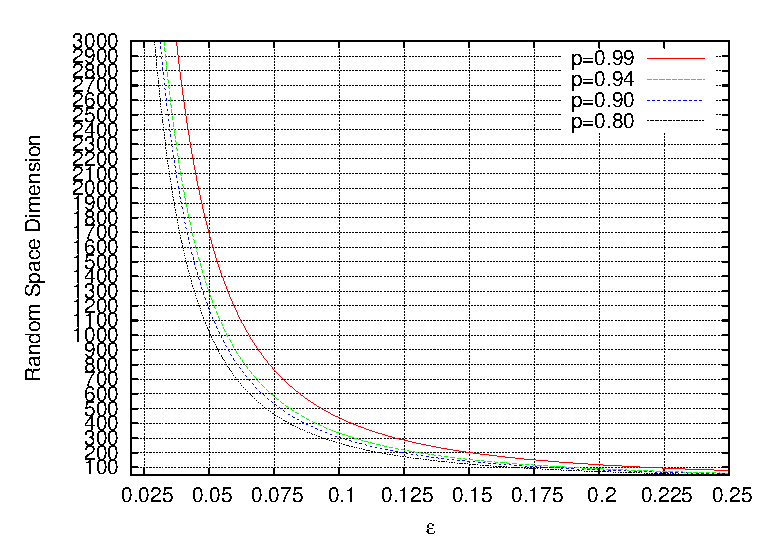
\includegraphics[scale=0.88]{tradeoffs1.eps}
	\end{figure}
\end{frame} 

\begin{frame}
\frametitle{Trade offs}
\framesubtitle{10 times more data}
 		\begin{figure}
		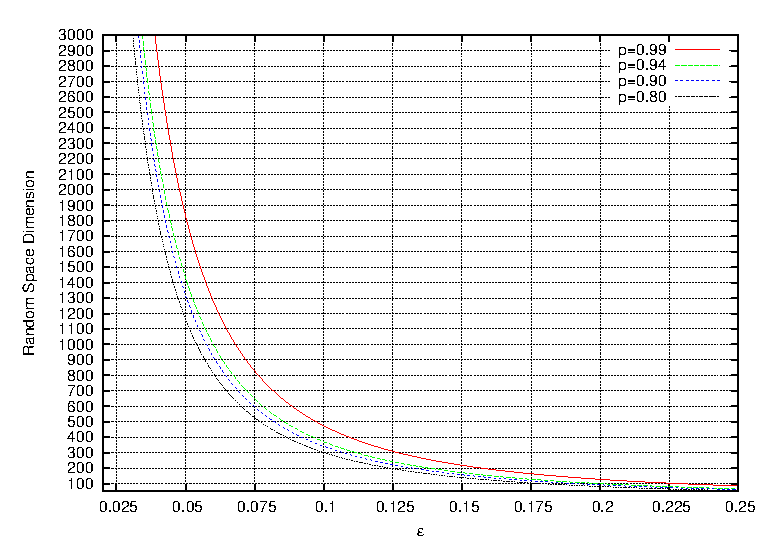
\includegraphics[scale=0.88]{tradeoffs2.eps}
	\end{figure}
\end{frame} 

\begin{frame}
\frametitle{Trade offs}
\framesubtitle{The effect of $n$}
 		\begin{figure}
		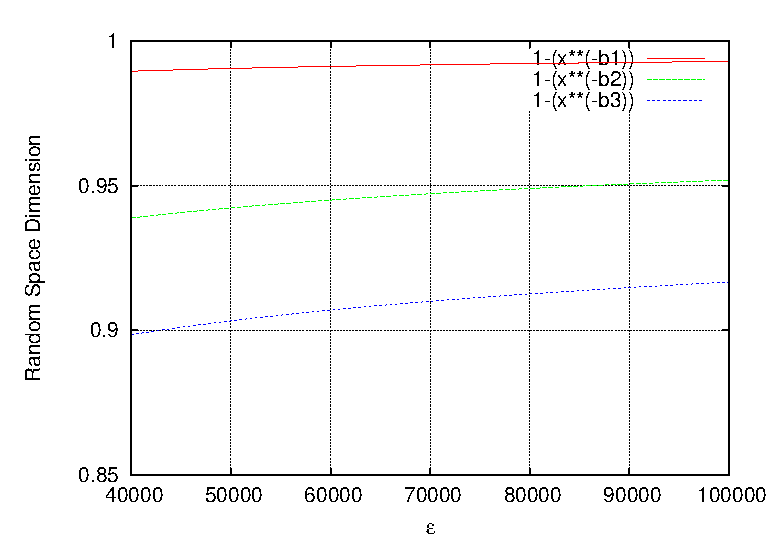
\includegraphics[scale=0.88]{tradeoffs3.eps}
	\end{figure}
\end{frame}

\section{Random Projections Design}

\begin{frame}
\frametitle{Random Projections Design}
\framesubtitle{Selecting $k_{0}$}

\begin{itemize}
  \item Determine how much data is available: $n$
  \item Compute $\beta$ for several certainty levels (99, 94, 90 typically)
  \item Compute and plot $k_{0}(\epsilon)$ for each $p$ level
  \item Choose $k_{0}$ according to resources constraints and accepted $\epsilon$
  \item More data? Start again. increase $k_{0}$, accept more error or more uncertainty
\end{itemize}
\end{frame} 


\begin{frame}
\frametitle{Random Projections Design}
\framesubtitle{Selecting a random distribution}

\begin{itemize}
  \item Select $k_{0}$ using a dense random distribution
  \item No $k_{0}$ meets performance criteria?: Analyze sparsity.
  \item If data is indeed really sparse, consider matrix densification algorithms
  \item If $k_{0}$ meets performance criteria, evaluate a sparse random projection
  \item Achlioptas' distributions are not the only meeting JL property. Others could give better results
\end{itemize}
\end{frame} 


\begin{frame}
\frametitle{Random Projections Design}
\framesubtitle{Weighting scheme}

\begin{itemize}
  \item Directional random vectors
  \item Distance permutations
  \item Reflective random projections
\end{itemize}
\end{frame} 

\section{High Level Metrics Correlations}
\begin{frame}
\frametitle{High Level Metrics Correlations}
\framesubtitle{Hit Ratio}
 		\begin{figure}
		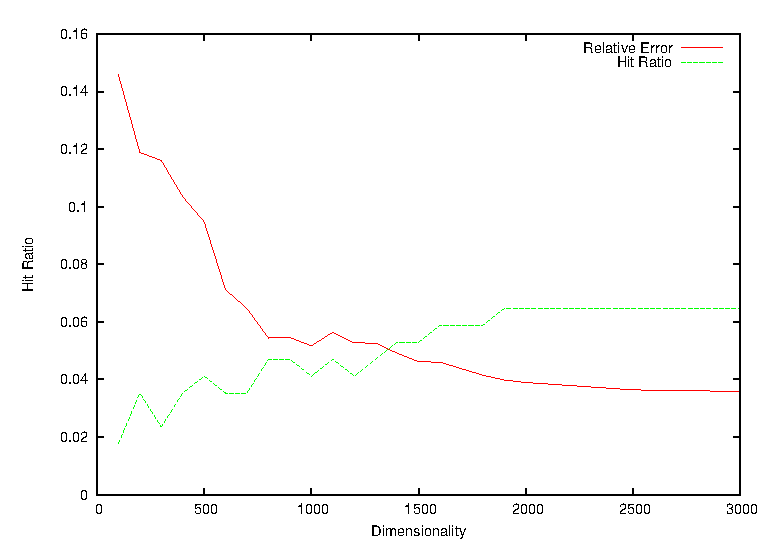
\includegraphics[scale=0.88]{hr.eps}
	\end{figure}
\end{frame}

\begin{frame}
\frametitle{High Level Metrics Correlations}
\framesubtitle{F-Score}
 		\begin{figure}
		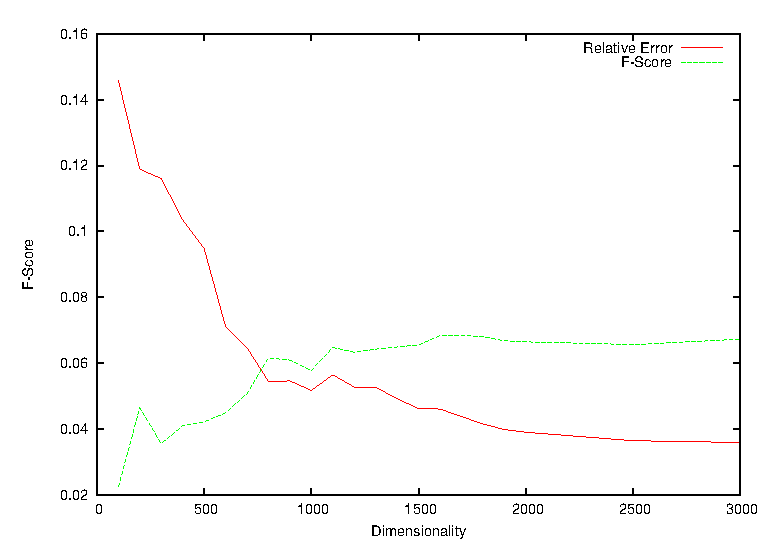
\includegraphics[scale=0.88]{fscore.eps}
	\end{figure}
\end{frame}


\begin{frame}
\frametitle{High Level Metrics Correlations}
\framesubtitle{Recall}
 		\begin{figure}
		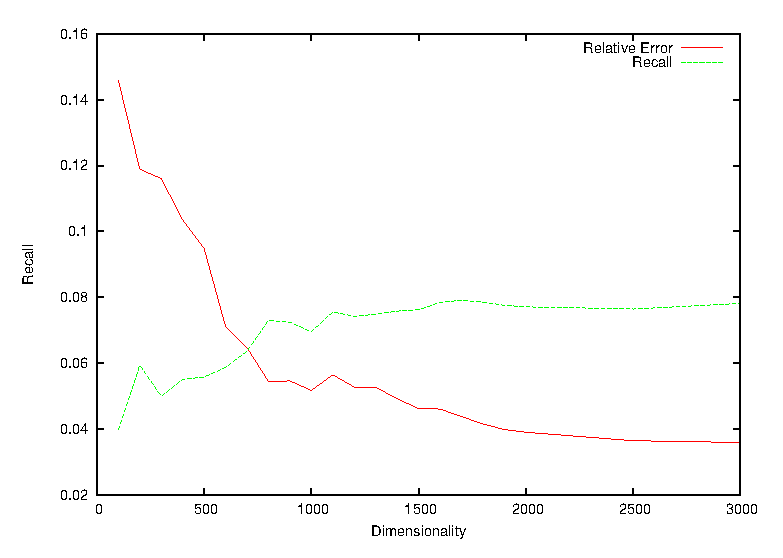
\includegraphics[scale=0.88]{recall.eps}
	\end{figure}
\end{frame}

\begin{frame}
\frametitle{High Level Metrics Correlations}
\framesubtitle{Recall}
 		\begin{figure}
		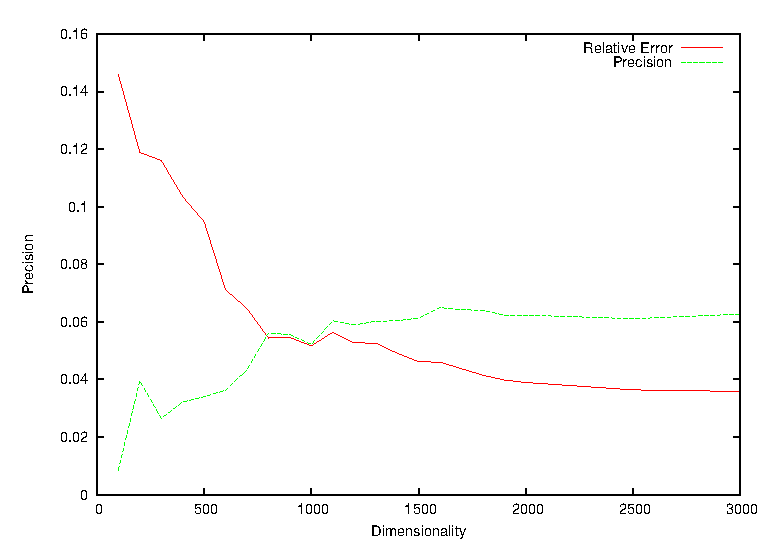
\includegraphics[scale=0.88]{precision.eps}
	\end{figure}
\end{frame}

\begin{frame}
\frametitle{High Level Metrics Correlations}
\framesubtitle{Recall}
 		\begin{figure}
		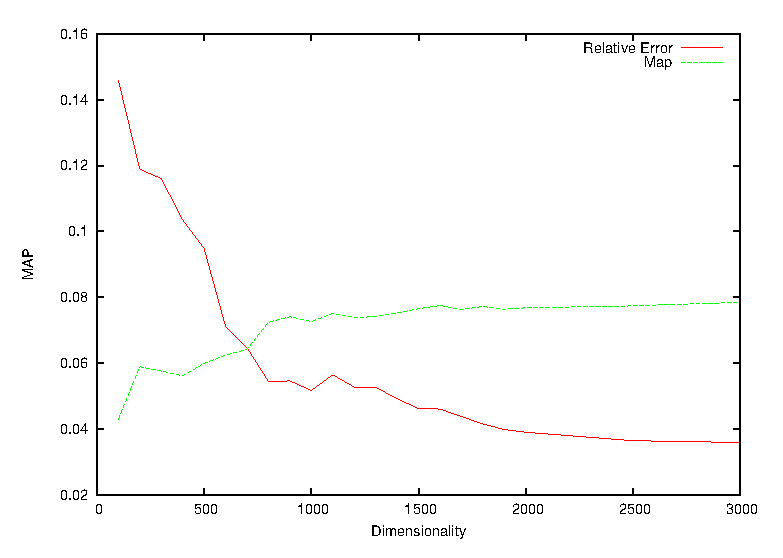
\includegraphics[scale=0.88]{map.eps}
	\end{figure}
\end{frame}

\section{Bibliography}
\begin{frame}%[allowframebreaks]
  \frametitle{Bibliography}    
  \begin{thebibliography}{10}
  \beamertemplatearticlebibitems
  \bibitem{Kanerva2000}
    P.~Kanerva, et al.
    \newblock {\em Random indexing of text samples for latent semantic analysis.}
    \newblock {\small Proceedings of the 22nd annual conference of the cognitive science society. Vol. 1036. 2000.}
  \beamertemplatearticlebibitems
  \bibitem{Achlioptas2003}
    D.~Achlioptas.
    \newblock {\em Database-friendly random projections: Johnson-Lindenstrauss with binary coins.}
    \newblock {\small Journal of computer and System Sciences 66.4 (2003): 671-687.}

  \bibitem{Venkatasubramanian2011}
    S.~Venkatasubramanian and Q.~Wang
    \newblock {\em The Johnson-Lindenstrauss Transform: An Empirical Study.}
    \newblock {\small ALENEX, pp. 164-173. 2011.}

  \bibitem{Sahlgren05}
    M.~Sahlgren
    \newblock {\em An introduction to random indexing}
    \newblock {\small In Methods and Applications of Semantic Indexing Workshop at the 7th International Conference on Terminology and Knowledge Engineering, TKE 2005}
  
    \bibitem{Sulic2010}
    V.~Sulic, J.~Per{\v{s}}, M.~Kristen and S.~Kovacic
    \newblock {\em Efficient dimensionality reduction using random projection}
    \newblock {\small Computer Vision Winter Workshop. 2010.}
    

  \end{thebibliography}
\end{frame}

\begin{frame}%[allowframebreaks]
  \frametitle{Bibliography}    
  \begin{thebibliography}{10}
  \beamertemplatearticlebibitems
  
  
    \bibitem{Sulic2010}
    V.~Sulic, J.~Per{\v{s}}, M.~Kristen and S.~Kovacic
    \newblock {\em Efficient dimensionality reduction using random projection}
    \newblock {\small Computer Vision Winter Workshop. 2010.}
    
        \bibitem{Sahlgren2008}
    M.~Sahlgren,  A.~Holst and P.~Kanerva
    \newblock {\em Permutations as a Means to Encode Order in Word Space}
    \newblock {\small Proceedings of the 30th Annual Conference of the Cognitive Science Society: 1300-1305.Computer Vision Winter Workshop. 2008.}

        \bibitem{Rangan2011}
    V.~Rangan
    \newblock {\em Discovery of related terms in a corpus using reflective random indexing}
    \newblock {\small Proceedings of Workshop on Setting Standards for Searching Electronically Stored Information In Discovery Proceedings (DESI-4). 2011.}
  \end{thebibliography}
  

\end{frame}

\begin{frame}%[allowframebreaks]
  \frametitle{Bibliography}    
  \begin{thebibliography}{10}
  \beamertemplatearticlebibitems
  
      
    \bibitem{Gorman2006}
    J.~Gorman and J.~Curran
    \newblock {\em Random indexing using statistical weight functions}
    \newblock {\small Proceedings of the 2006 Conference on Empirical Methods in Natural Language Processing, pp. 457-464. Association for Computational Linguistics, 2006.}
  
        
    \bibitem{Sahlgren2006}
    M.~Sahlgren
    \newblock {\em The Word-Space Model: Using distributional analysis to represent syntagmatic and paradigmatic relations between words in high-dimensional vector spaces.}
    \newblock {\small Diss. Stockholm, 2006.}
  \end{thebibliography}

\end{frame}



\end{document}
